% !TeX program = xelatex
\documentclass[a4paper,10pt]{article}

% ============================================================================
% កញ្ចប់បណ្ណាល័យ (Packages) – តាមលំនាំ NGS Preah Krasang (ls_plan.tex)
% ============================================================================
\usepackage[a4paper, left=0.95cm, right=0.95cm, top=0.85cm, bottom=0.92cm, footskip=0.52cm]{geometry}
\usepackage{amsmath, amssymb}
\usepackage{unicode-math}
\usepackage{fontspec}
\usepackage{array, longtable, multirow, colortbl}
\usepackage[table]{xcolor}
\usepackage{enumitem}
\usepackage{pifont}
\usepackage{fancyhdr}
\usepackage{tikz}
\usetikzlibrary{calc, arrows.meta, decorations.markings, decorations.pathreplacing, patterns, babel}

% LaTeX 2025 + longtable v4.24 compatibility guard
\makeatletter
\let\@expl@@@mark@update@singlecol@structures@@\relax
\makeatother

% ============================================================================
% ការកំណត់ពុម្ពអក្សរ (Cross-Platform Fonts Configuration)
% ============================================================================
\providecommand{\NGSFindFonts}{%
  \IfFileExists{C:/Windows/Fonts/cambria.ttc}{%
    \def\NGSSysPath{C:/Windows/Fonts/}%
    \def\NGSUserPath{C:/Users/KIT/AppData/Local/Microsoft/Windows/Fonts/}%
  }{%
    \IfFileExists{./fonts/KhmerOSsiemreap.ttf}{\def\NGSSysPath{./fonts/}\def\NGSUserPath{./fonts/}}{%
    \IfFileExists{../fonts/KhmerOSsiemreap.ttf}{\def\NGSSysPath{../fonts/}\def\NGSUserPath{../fonts/}}{%
    \IfFileExists{../../fonts/KhmerOSsiemreap.ttf}{\def\NGSSysPath{../../fonts/}\def\NGSUserPath{../../fonts/}}{%
    \IfFileExists{../../../fonts/KhmerOSsiemreap.ttf}{\def\NGSSysPath{../../../fonts/}\def\NGSUserPath{../../../fonts/}}{%
    \IfFileExists{../../../../fonts/KhmerOSsiemreap.ttf}{\def\NGSSysPath{../../../../fonts/}\def\NGSUserPath{../../../../fonts/}}{%
    \IfFileExists{../../../../../fonts/KhmerOSsiemreap.ttf}{\def\NGSSysPath{../../../../../fonts/}\def\NGSUserPath{../../../../../fonts/}}{%
    \IfFileExists{../../../../../../fonts/KhmerOSsiemreap.ttf}{\def\NGSSysPath{../../../../../../fonts/}\def\NGSUserPath{../../../../../../fonts/}}{%
      \def\NGSSysPath{../../../../../../../fonts/}\def\NGSUserPath{../../../../../../../fonts/}%
    }}}}}}}%
  }%
}
\NGSFindFonts

\setmathfont[
  Path={\NGSSysPath},
  FontIndex=1,
  Scale=1.02
]{cambria.ttc}

\defaultfontfeatures{Ligatures=TeX}

\setmainfont[
  Path={\NGSUserPath},
  Extension=.ttf,
  Script=Khmer,
  BoldFont={KhmerOSsiemreap},
  BoldFeatures={FakeBold=1.8},
  ItalicFont={KhmerOSsiemreap},
  ItalicFeatures={FakeSlant=0.25},
  BoldItalicFont={KhmerOSsiemreap},
  BoldItalicFeatures={FakeBold=1.8, FakeSlant=0.25}
]{KhmerOSsiemreap}

\newfontfamily\muol[
  Path={\NGSUserPath},
  Extension=.ttf,
  Script=Khmer
]{KhmerOSmuollight}

\newfontfamily\TimesEn[
  Path={\NGSSysPath},
  Extension=.ttf,
  Scale=1.00,
  BoldFont={timesbd},
  ItalicFont={timesi},
  BoldItalicFont={timesbi}
]{times}

\newfontfamily\NagaBold[
  Path={\NGSUserPath},
  Extension=.ttf
]{AKbalthom Naga Bold}

\newfontfamily\CalibriFont[
  Path={\NGSSysPath},
  Extension=.ttf
]{calibri}

\newfontfamily\Tacteing[
  Path={\NGSUserPath}
]{TACTENG.TTF}

\newfontfamily\CourierBullet[
  Path={\NGSSysPath},
  Extension=.ttf
]{cour}
\newcommand{\wcirc}{{\CourierBullet\fontsize{9.5pt}{11pt}\selectfont o}}

% ក្បួនកាត់ពាក្យខ្មែរ (Khmer word wrapping)
\XeTeXlinebreaklocale "km"
\XeTeXlinebreakskip = 0pt plus 1pt minus 0.1pt

% ============================================================================
% ការកំណត់ពណ៌ និងទម្រង់ទំព័រ (Colors & Page Style)
% ============================================================================
\definecolor{stepgray}{HTML}{D9D9D9}
\definecolor{headgray}{HTML}{F2F2F2}
\definecolor{boxgray}{HTML}{D9D9D9}
\definecolor{darkred}{HTML}{C00000}
\definecolor{red5e}{HTML}{FF0000}

\pagestyle{fancy}
\fancyhf{}
\renewcommand{\headrulewidth}{0pt}
\fancyfoot[R]{\CalibriFont\fontsize{11pt}{13pt}\selectfont\thepage}

\setlength{\parindent}{0pt}
\setlength{\parskip}{0pt}
\setlength{\tabcolsep}{3.8pt}

\newcolumntype{L}[1]{>{\raggedright\arraybackslash}p{#1}}

% ============================================================================
% ម៉ាក្រូជំនួយ (Helper Macros)
% ============================================================================
\newcommand{\en}[1]{{\TimesEn #1}}
\newcommand{\enbf}[1]{{\TimesEn\textbf{#1}}}
\newcommand{\unit}[1]{\,\text{\en{#1}}}
\newcommand{\fiveE}[1]{{\NagaBold\fontsize{9.5pt}{13pt}\selectfont\textcolor{red5e}{#1}}}
\newcommand{\timenote}[1]{\textcolor{darkred}{\textit{#1}}}
\newcommand{\redsub}[1]{\textcolor{darkred}{#1}}
\newcommand{\graybox}[1]{\colorbox{boxgray}{\strut\hspace{2pt}#1\hspace{2pt}}}
\newcommand{\ditem}{\tikz[baseline=-0.5ex]\fill (0,0.42ex) -- (0.42ex,0) -- (0,-0.42ex) -- (-0.42ex,0) -- cycle;\hspace{0.3em}}
\newcommand{\cnum}[1]{{\fontsize{10.5pt}{12pt}\selectfont\ding{\numexpr181+#1\relax}}\hspace{0.15em}}
\newcommand{\cfig}[1]{\par\vspace{2pt}{\centering #1\par}\vspace{2pt}}
\newcommand{\stepheader}[1]{\multicolumn{3}{|c|}{\cellcolor{stepgray}\muol #1} \\* \noalign{\hrule height 0.4pt}}
\newcommand{\khmflourish}{{\Tacteing\fontsize{36pt}{14pt}\selectfont\raisebox{-5pt}{3}}}

% ============================================================================
% ម៉ាក្រូគូសរូប TikZ ស-ខ្មៅ (3.8–7.3 cm, អក្សរខ្មៅ 100%, >=8.5pt \footnotesize)
% ============================================================================

% ១. ជំហានទី២.១៖ កំណែកិច្ចការផ្ទះ (ទំ.២៥ លំហាត់ទី៦ ក, ខ, គ)
\newcommand{\figHWoldPOW}{%
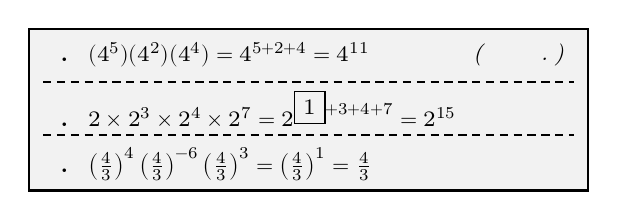
\begin{tikzpicture}[scale=1.0, every node/.style={font=\footnotesize, text=black}]
  \draw[black, line width=0.95pt, fill=gray!10] (0,0) rectangle (7.10, 2.05);
  \node[anchor=west] at (0.20, 1.72) {\textbf{៦.ក}\; $(4^5)(4^2)(4^4) = 4^{5+2+4} = 4^{11}$};
  \draw[black, densely dashed, line width=0.7pt] (0.18, 1.38) -- (6.92, 1.38);
  \node[anchor=west] at (0.20, 1.04) {\textbf{៦.ខ}\; $2\times 2^3\times 2^4\times 2^7 = 2^{\boxed{1}+3+4+7} = 2^{15}$};
  \draw[black, densely dashed, line width=0.7pt] (0.18, 0.70) -- (6.92, 0.70);
  \node[anchor=west] at (0.20, 0.34) {\textbf{៦.គ}\; $\left(\frac{4}{3}\right)^4\left(\frac{4}{3}\right)^{-6}\left(\frac{4}{3}\right)^3 = \left(\frac{4}{3}\right)^1 = \frac{4}{3}$};
  \node[anchor=east] at (6.92, 1.72) {\textit{(កុំដាក់ ៦.ឃ)}};
\end{tikzpicture}}

% ២. ជំហានទី២.២៖ រំលឹកចំណេះមូលដ្ឋាន (k/k=1, x=x^1, ដករ៉ឺឡាទីប)
\newcommand{\figPrereqPOW}{%
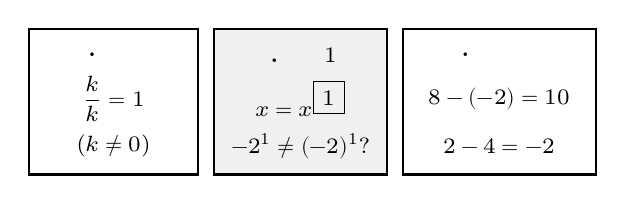
\begin{tikzpicture}[scale=1.0, every node/.style={font=\footnotesize, text=black}]
  % ប្រអប់ ១
  \draw[black, line width=0.9pt, fill=white] (0,0) rectangle (2.15, 1.85);
  \node at (1.075, 1.52) {\textbf{១. សម្រួល}};
  \node at (1.075, 0.96) {$\dfrac{k}{k} = 1$};
  \node at (1.075, 0.36) {($k \neq 0$)};
  % ប្រអប់ ២
  \draw[black, line width=0.9pt, fill=gray!12] (2.35,0) rectangle (4.55, 1.85);
  \node at (3.45, 1.52) {\textbf{២. លាក់ $1$}};
  \node at (3.45, 0.96) {$x = x^{\boxed{1}}$};
  \node at (3.45, 0.36) {$-2^1 \neq (-2)^1$?};
  % ប្រអប់ ៣
  \draw[black, line width=0.9pt, fill=white] (4.75,0) rectangle (7.20, 1.85);
  \node at (5.975, 1.52) {\textbf{៣. ដករ៉ឺឡាទីប}};
  \node at (5.975, 0.96) {$8 - (-2) = 10$};
  \node at (5.975, 0.36) {$2 - 4 = -2$};
\end{tikzpicture}}

% ៣. ជំហានទី២.៣ E1 Engage: ឃ្លាំងផ្ទុកទិន្នន័យសាលាឌីជីថល NGS
\newcommand{\figEngagePOW}{%
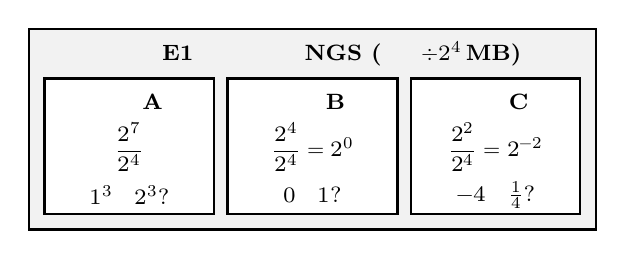
\begin{tikzpicture}[scale=1.0, every node/.style={font=\footnotesize, text=black}]
  \draw[black, line width=0.95pt, fill=gray!10] (0,0) rectangle (7.20, 2.55);
  \node at (3.60, 2.24) {\textbf{បេសកកម្ម \en{E1}៖ ឃ្លាំងទិន្នន័យ \en{NGS} (បំបែក $\div 2^4\unit{MB}$)}};
  % បន្ទប់ A
  \draw[black, line width=0.95pt, fill=white] (0.20, 0.20) rectangle (2.35, 1.92);
  \node at (1.275, 1.62) {\textbf{បន្ទប់ \en{A}}};
  \node at (1.275, 1.05) {$\dfrac{2^7}{2^4}$};
  \node at (1.275, 0.44) {$1^3$ ឬ $2^3$?};
  % បន្ទប់ B
  \draw[black, line width=0.95pt, fill=white] (2.52, 0.20) rectangle (4.68, 1.92);
  \node at (3.60, 1.62) {\textbf{បន្ទប់ \en{B}}};
  \node at (3.60, 1.05) {$\dfrac{2^4}{2^4} = 2^0$};
  \node at (3.60, 0.44) {$0$ ឬ $1$?};
  % បន្ទប់ C
  \draw[black, line width=0.95pt, fill=white] (4.85, 0.20) rectangle (7.00, 1.92);
  \node at (5.925, 1.62) {\textbf{បន្ទប់ \en{C}}};
  \node at (5.925, 1.05) {$\dfrac{2^2}{2^4} = 2^{-2}$};
  \node at (5.925, 0.44) {$-4$ ឬ $\frac{1}{4}$?};
\end{tikzpicture}}

% ៤ក. E2 Act 1 កញ្ចប់ A: បន្ទះកាត់ 1:1 ២^7 / ២^4 (ពេញ ៧ កត្តា — កែសៀវភៅទំ.១៦)
\newcommand{\figExploreOneAPOW}{%
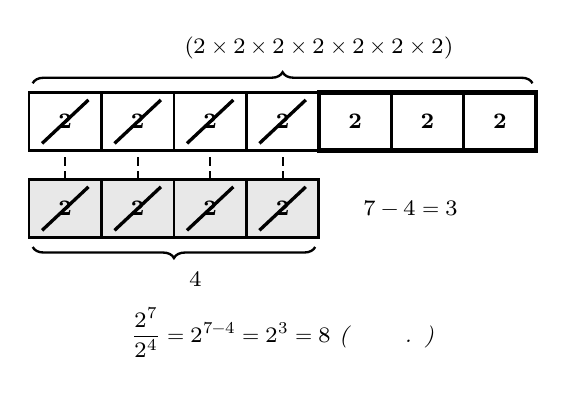
\begin{tikzpicture}[scale=0.92, every node/.style={font=\footnotesize, text=black}]
  % ភាគយក ៧ ប្រអប់ពេញ (0..7)
  \foreach \i in {0,...,6}{
    \draw[black, line width=1.0pt, fill=white] (\i, 1.45) rectangle (\i+1, 2.25);
    \node at (\i+0.5, 1.85) {$\mathbf{2}$};
  }
  % ភាគបែង ៤ ប្រអប់ (0..4) + សញ្ញាឈូសសម្រួល ១-ទល់-១
  \foreach \i in {0,...,3}{
    \draw[black, line width=1.0pt, fill=gray!18] (\i, 0.25) rectangle (\i+1, 1.05);
    \node at (\i+0.5, 0.65) {$\mathbf{2}$};
    \draw[black, densely dashed, line width=0.75pt] (\i+0.5, 1.05) -- (\i+0.5, 1.45);
    \draw[black, line width=1.2pt] (\i+0.18, 1.55) -- (\i+0.82, 2.15);
    \draw[black, line width=1.2pt] (\i+0.18, 0.35) -- (\i+0.82, 0.95);
  }
  % ស៊ុមក្រាស់ជុំវិញកត្តា ៣ ដែលនៅសល់
  \draw[black, line width=1.6pt] (4.0, 1.45) rectangle (7.0, 2.25);
  % ដង្កៀបលើ និង ក្រោម
  \draw[black, decorate, decoration={brace, amplitude=4pt}, line width=0.85pt] (0.05, 2.38) -- (6.95, 2.38)
    node[midway, above=5pt] {\textbf{៧ កត្តាពេញ} ($2\times 2\times 2\times 2\times 2\times 2\times 2$)};
  \draw[black, decorate, decoration={brace, amplitude=4pt, mirror}, line width=0.85pt] (0.05, 0.12) -- (3.95, 0.12)
    node[midway, below=5pt] {សម្រួលអស់ $4$ គូ};
  \node[anchor=west] at (4.12, 0.65) {សល់ $7-4 = 3$ កត្តា};
  \node at (3.50, -1.06) {$\dfrac{2^7}{2^4} = 2^{7-4} = 2^3 = 8$ \textit{(កែសៀវភៅទំ.១៦)}};
\end{tikzpicture}}

% ៤ខ. E2 Act 1 កញ្ចប់ B: បន្ទះកាត់ 1:1 ៣^7 / ៣^5
\newcommand{\figExploreOneBPOW}{%
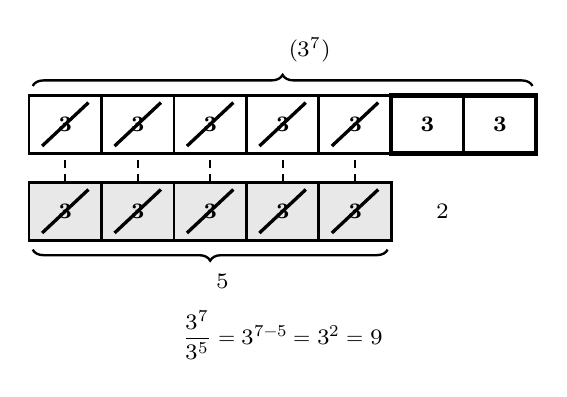
\begin{tikzpicture}[scale=0.92, every node/.style={font=\footnotesize, text=black}]
  \foreach \i in {0,...,6}{
    \draw[black, line width=1.0pt, fill=white] (\i, 1.45) rectangle (\i+1, 2.25);
    \node at (\i+0.5, 1.85) {$\mathbf{3}$};
  }
  \foreach \i in {0,...,4}{
    \draw[black, line width=1.0pt, fill=gray!18] (\i, 0.25) rectangle (\i+1, 1.05);
    \node at (\i+0.5, 0.65) {$\mathbf{3}$};
    \draw[black, densely dashed, line width=0.75pt] (\i+0.5, 1.05) -- (\i+0.5, 1.45);
    \draw[black, line width=1.2pt] (\i+0.18, 1.55) -- (\i+0.82, 2.15);
    \draw[black, line width=1.2pt] (\i+0.18, 0.35) -- (\i+0.82, 0.95);
  }
  \draw[black, line width=1.6pt] (5.0, 1.45) rectangle (7.0, 2.25);
  \draw[black, decorate, decoration={brace, amplitude=4pt}, line width=0.85pt] (0.05, 2.38) -- (6.95, 2.38)
    node[midway, above=5pt] {\textbf{៧ កត្តា} ($3^7$)};
  \draw[black, decorate, decoration={brace, amplitude=4pt, mirror}, line width=0.85pt] (0.05, 0.12) -- (4.95, 0.12)
    node[midway, below=5pt] {សម្រួល $5$ គូ};
  \node[anchor=west] at (5.12, 0.65) {សល់ $2$ កត្តា};
  \node at (3.50, -1.06) {$\dfrac{3^7}{3^5} = 3^{7-5} = 3^2 = 9$};
\end{tikzpicture}}

% ៥ក. E2 Act 2 Dual POE 2A (m=n) & 2B (m<n)
\newcommand{\figExploreTwoAPOW}{%
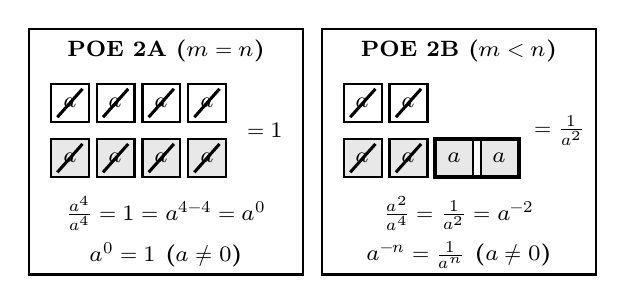
\begin{tikzpicture}[scale=1.0, every node/.style={font=\footnotesize, text=black}]
  % 2A Panel
  \begin{scope}[shift={(0,0)}]
    \draw[black, line width=0.95pt, fill=white] (0,0) rectangle (3.48, 3.12);
    \node at (1.74, 2.84) {\textbf{POE 2A ($m=n$)}};
    \foreach \i in {0,...,3}{
      \draw[black, line width=0.85pt, fill=white] (0.28+\i*0.58, 1.94) rectangle (0.76+\i*0.58, 2.42);
      \node at (0.52+\i*0.58, 2.18) {$a$};
      \draw[black, line width=0.85pt, fill=gray!18] (0.28+\i*0.58, 1.24) rectangle (0.76+\i*0.58, 1.72);
      \node at (0.52+\i*0.58, 1.48) {$a$};
      \draw[black, line width=1.1pt] (0.36+\i*0.58, 2.00) -- (0.68+\i*0.58, 2.36);
      \draw[black, line width=1.1pt] (0.36+\i*0.58, 1.30) -- (0.68+\i*0.58, 1.66);
    }
    \node at (3.00, 1.83) {$= 1$};
    \node at (1.74, 0.78) {$\tfrac{a^4}{a^4} = 1 = a^{4-4} = a^0$};
    \node at (1.74, 0.25) {\textbf{$a^0 = 1$ ($a\neq 0$)}};
  \end{scope}
  % 2B Panel
  \begin{scope}[shift={(3.72,0)}]
    \draw[black, line width=0.95pt, fill=white] (0,0) rectangle (3.48, 3.12);
    \node at (1.74, 2.84) {\textbf{POE 2B ($m<n$)}};
    \foreach \i in {0,1}{
      \draw[black, line width=0.85pt, fill=white] (0.28+\i*0.58, 1.94) rectangle (0.76+\i*0.58, 2.42);
      \node at (0.52+\i*0.58, 2.18) {$a$};
      \draw[black, line width=1.1pt] (0.36+\i*0.58, 2.00) -- (0.68+\i*0.58, 2.36);
    }
    \foreach \i in {0,...,3}{
      \draw[black, line width=0.85pt, fill=gray!18] (0.28+\i*0.58, 1.24) rectangle (0.76+\i*0.58, 1.72);
      \node at (0.52+\i*0.58, 1.48) {$a$};
    }
    \foreach \i in {0,1}{
      \draw[black, line width=1.1pt] (0.36+\i*0.58, 1.30) -- (0.68+\i*0.58, 1.66);
    }
    \draw[black, line width=1.45pt] (1.44, 1.24) rectangle (2.50, 1.72);
    \node at (3.02, 1.83) {$= \frac{1}{a^2}$};
    \node at (1.74, 0.78) {$\tfrac{a^2}{a^4} = \tfrac{1}{a^2} = a^{-2}$};
    \node at (1.74, 0.25) {\textbf{$a^{-n} = \frac{1}{a^n}$ ($a\neq 0$)}};
  \end{scope}
\end{tikzpicture}}

% ៥ខ. E2 Act 2: ជណ្ដើរស្វ័យគុណ (Exponent Ladder: a^3 -> a^{-2}, ÷a)
\newcommand{\figExploreTwoBPOW}{%
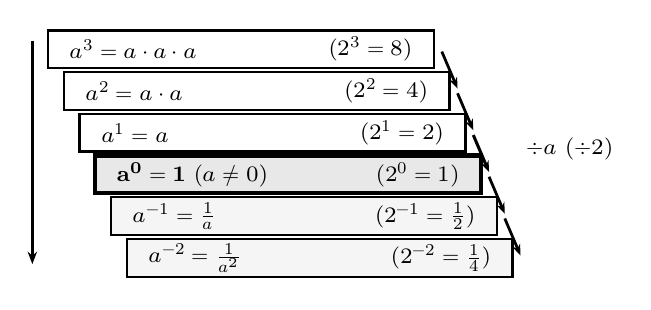
\begin{tikzpicture}[scale=1.0, every node/.style={font=\footnotesize, text=black}]
  \draw[black, line width=0.9pt, fill=white] (0.35, 2.65) rectangle (5.25, 3.13);
  \node[anchor=west] at (0.50, 2.89) {$a^3 = a\cdot a\cdot a$};
  \node[anchor=east] at (5.10, 2.89) {($2^3 = 8$)};

  \draw[black, line width=0.9pt, fill=white] (0.55, 2.12) rectangle (5.45, 2.60);
  \node[anchor=west] at (0.70, 2.36) {$a^2 = a\cdot a$};
  \node[anchor=east] at (5.30, 2.36) {($2^2 = 4$)};

  \draw[black, line width=0.9pt, fill=white] (0.75, 1.59) rectangle (5.65, 2.07);
  \node[anchor=west] at (0.90, 1.83) {$a^1 = a$};
  \node[anchor=east] at (5.50, 1.83) {($2^1 = 2$)};

  \draw[black, line width=1.45pt, fill=gray!18] (0.95, 1.06) rectangle (5.85, 1.54);
  \node[anchor=west] at (1.10, 1.30) {$\mathbf{a^0 = 1}$ ($a\neq 0$)};
  \node[anchor=east] at (5.70, 1.30) {($2^0 = 1$)};

  \draw[black, line width=0.9pt, fill=gray!8] (1.15, 0.53) rectangle (6.05, 1.01);
  \node[anchor=west] at (1.30, 0.77) {$a^{-1} = \frac{1}{a}$};
  \node[anchor=east] at (5.90, 0.77) {($2^{-1} = \frac{1}{2}$)};

  \draw[black, line width=0.9pt, fill=gray!8] (1.35, 0.00) rectangle (6.25, 0.48);
  \node[anchor=west] at (1.50, 0.24) {$a^{-2} = \frac{1}{a^2}$};
  \node[anchor=east] at (6.10, 0.24) {($2^{-2} = \frac{1}{4}$)};

  % ព្រួញចុះ ÷a ខាងស្ដាំ និងព្រួញឆ្វេង
  \draw[black, line width=1.0pt, -{Stealth[length=4pt]}] (5.35, 2.86) -- (5.55, 2.39);
  \draw[black, line width=1.0pt, -{Stealth[length=4pt]}] (5.55, 2.33) -- (5.75, 1.86);
  \draw[black, line width=1.1pt, -{Stealth[length=4pt]}] (5.75, 1.80) -- (5.95, 1.33);
  \draw[black, line width=1.0pt, -{Stealth[length=4pt]}] (5.95, 1.27) -- (6.15, 0.80);
  \draw[black, line width=1.0pt, -{Stealth[length=4pt]}] (6.15, 0.74) -- (6.35, 0.27);
  \node[anchor=west] at (6.30, 1.62) {$\div a$ ($\div 2$)};
  \draw[black, line width=1.05pt, -{Stealth[length=4.5pt]}] (0.15, 3.00) -- (0.15, 0.16);
\end{tikzpicture}}

% ៦. E3 Explain: កាតប្រៀបធៀប (-2)^6 vs -2^6 និងការពារដែនកំណត់ a≠0
\newcommand{\figExplainParensPOW}{%
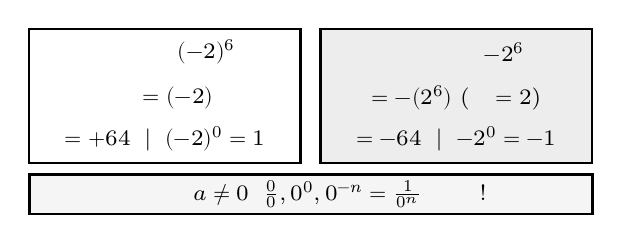
\begin{tikzpicture}[scale=1.0, every node/.style={font=\footnotesize, text=black}]
  \draw[black, line width=0.95pt, fill=white] (0, 0.65) rectangle (3.45, 2.35);
  \node at (1.725, 2.06) {\textbf{មានវង់ក្រចក៖ $(-2)^6$}};
  \node at (1.725, 1.48) {គោល $= (-2)$};
  \node at (1.725, 0.95) {$= +64$ \;\textbar{}\; $(-2)^0 = 1$};

  \draw[black, line width=0.95pt, fill=gray!14] (3.70, 0.65) rectangle (7.15, 2.35);
  \node at (5.425, 2.06) {\textbf{គ្មានវង់ក្រចក៖ $-2^6$}};
  \node at (5.425, 1.48) {$= -(2^6)$ (គោល $= 2$)};
  \node at (5.425, 0.95) {$= -64$ \;\textbar{}\; $-2^0 = -1$};

  \draw[black, line width=1.05pt, fill=gray!8] (0, 0) rectangle (7.15, 0.50);
  \node at (3.575, 0.25) {\textbf{ដែនកំណត់ $a\neq 0$៖} $\frac{0}{0}, 0^0, 0^{-n} = \frac{1}{0^n}$ គ្មានន័យ!};
\end{tikzpicture}}

% ៧. E4 Elaborate: កាតស៊ើបអង្កេត B&W [tracing] — លំហាត់គំរូ គ (ទំ.១៦)
\newcommand{\figModelTracingPOW}{%
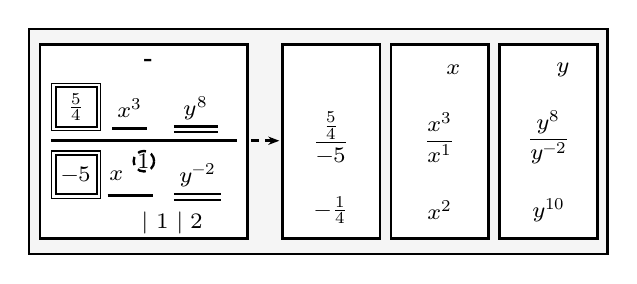
\begin{tikzpicture}[scale=1.0, every node/.style={font=\footnotesize, text=black}]
  \draw[black, line width=0.9pt, fill=gray!8] (0,0) rectangle (7.35, 2.86);
  % កន្សោមដើមខាងឆ្វេង
  \draw[black, line width=1.0pt, fill=white] (0.14, 0.20) rectangle (2.78, 2.66);
  \node at (1.46, 2.44) {\textbf{កូដ ស-ខ្មៅ}};
  \draw[black, line width=0.9pt] (0.28, 1.44) -- (2.64, 1.44);
  % ភាគយក
  \draw[black, line width=0.75pt] (0.34, 1.62) rectangle (0.86, 2.12);
  \draw[black, line width=0.45pt] (0.29, 1.57) rectangle (0.91, 2.17);
  \node at (0.60, 1.87) {$\frac{5}{4}$};
  \node at (1.28, 1.85) {$x^3$};
  \draw[black, line width=1.15pt] (1.06, 1.60) -- (1.50, 1.60);
  \node at (2.12, 1.85) {$y^8$};
  \draw[black, line width=0.8pt] (1.84, 1.62) -- (2.40, 1.62) (1.84, 1.55) -- (2.40, 1.55);
  % ភាគបែង
  \draw[black, line width=0.75pt] (0.34, 0.76) rectangle (0.86, 1.26);
  \draw[black, line width=0.45pt] (0.29, 0.71) rectangle (0.91, 1.31);
  \node at (0.60, 1.01) {$-5$};
  \node at (1.12, 1.00) {$x$};
  \draw[black, line width=0.85pt, densely dashed] (1.46, 1.18) circle (0.13);
  \node at (1.46, 1.18) {$1$};
  \draw[black, line width=1.15pt] (1.00, 0.74) -- (1.58, 0.74);
  \node at (2.14, 1.00) {$y^{-2}$};
  \draw[black, line width=0.8pt] (1.84, 0.76) -- (2.44, 0.76) (1.84, 0.69) -- (2.44, 0.69);
  \node at (1.46, 0.40) {ស៊ុមទ្វេ \textbar{} $1$ \textbar{} $2$};

  % ព្រួញ [tracing]
  \draw[black, densely dashed, line width=1.0pt, -{Stealth[length=4pt]}] (2.82, 1.44) -- (3.18, 1.44);

  % ៣ ក្រុមខាងស្ដាំ
  \draw[black, line width=0.95pt, fill=white] (3.22, 0.20) rectangle (4.46, 2.66);
  \node at (3.84, 2.34) {\textbf{មេគុណ}};
  \node at (3.84, 1.48) {$\dfrac{\frac{5}{4}}{-5}$};
  \node at (3.84, 0.56) {$-\frac{1}{4}$};

  \draw[black, line width=0.95pt, fill=white] (4.60, 0.20) rectangle (5.84, 2.66);
  \node at (5.22, 2.34) {\textbf{គោល $x$}};
  \node at (5.22, 1.48) {$\dfrac{x^3}{x^1}$};
  \node at (5.22, 0.56) {$x^{2}$};

  \draw[black, line width=0.95pt, fill=white] (5.98, 0.20) rectangle (7.22, 2.66);
  \node at (6.60, 2.34) {\textbf{គោល $y$}};
  \node at (6.60, 1.48) {$\dfrac{y^8}{y^{-2}}$};
  \node at (6.60, 0.56) {$y^{10}$};
\end{tikzpicture}}

% ៨. E5 Evaluate: កាតវិនិច្ឆ័យរហ័ស A–D បំបែកជា ២ ជួរ (A-B និង C-D)
\newcommand{\figExitFoilABPOW}{%
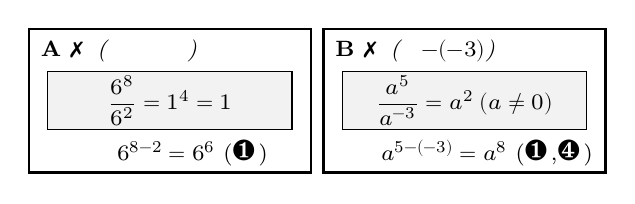
\begin{tikzpicture}[scale=1.0, every node/.style={font=\footnotesize, text=black}]
  \begin{scope}[shift={(0,0)}]
    \draw[black, line width=0.95pt, fill=white] (0,0) rectangle (3.58, 1.82);
    \node[anchor=north west, inner sep=3pt] at (0.04, 1.79) {\textbf{\en{A} \ding{55}} \;\textit{(អន្ទាក់ចែកគោល)}};
    \draw[black, fill=gray!10] (0.24, 0.54) rectangle (3.34, 1.28);
    \node at (1.79, 0.91) {$\dfrac{6^8}{6^2} = 1^4 = 1$};
    \node at (1.79, 0.24) {ត្រូវ៖ $6^{8-2} = 6^6$ (\cnum{1})};
  \end{scope}
  \begin{scope}[shift={(3.74,0)}]
    \draw[black, line width=0.95pt, fill=white] (0,0) rectangle (3.58, 1.82);
    \node[anchor=north west, inner sep=3pt] at (0.04, 1.79) {\textbf{\en{B} \ding{55}} \;\textit{(ដក $-(-3)$)}};
    \draw[black, fill=gray!10] (0.24, 0.54) rectangle (3.34, 1.28);
    \node at (1.79, 0.91) {$\dfrac{a^5}{a^{-3}} = a^2\;(a\neq 0)$};
    \node at (1.79, 0.24) {ត្រូវ៖ $a^{5-(-3)} = a^8$ (\cnum{1},\cnum{4})};
  \end{scope}
\end{tikzpicture}}

\newcommand{\figExitFoilCDPOW}{%
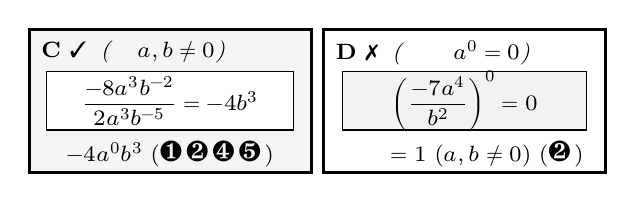
\begin{tikzpicture}[scale=1.0, every node/.style={font=\footnotesize, text=black}]
  \begin{scope}[shift={(0,0)}]
    \draw[black, line width=1.15pt, fill=gray!8] (0,0) rectangle (3.58, 1.82);
    \node[anchor=north west, inner sep=3pt] at (0.04, 1.79) {\textbf{\en{C} \ding{51}} \;\textit{(ពិត $a,b\neq 0$)}};
    \draw[black, fill=white] (0.22, 0.54) rectangle (3.36, 1.28);
    \node at (1.79, 0.91) {$\dfrac{-8a^3 b^{-2}}{2a^3 b^{-5}} = -4b^3$};
    \node at (1.79, 0.24) {$-4a^0b^3$ (\cnum{1}\cnum{2}\cnum{4}\cnum{5})};
  \end{scope}
  \begin{scope}[shift={(3.74,0)}]
    \draw[black, line width=0.95pt, fill=white] (0,0) rectangle (3.58, 1.82);
    \node[anchor=north west, inner sep=3pt] at (0.04, 1.79) {\textbf{\en{D} \ding{55}} \;\textit{(អន្ទាក់ $a^0=0$)}};
    \draw[black, fill=gray!10] (0.24, 0.54) rectangle (3.34, 1.28);
    \node at (1.79, 0.91) {$\left(\dfrac{-7a^4}{b^2}\right)^0 = 0$};
    \node at (1.79, 0.24) {ត្រូវ៖ $= 1$ ($a,b\neq 0$) (\cnum{2})};
  \end{scope}
\end{tikzpicture}}

% ============================================================================
% ចាប់ផ្ដើមឯកសារ (Document Body)
% ============================================================================
\begin{document}
\fontsize{10pt}{15.2pt}\selectfont

% -------------------- ក្បាលកិច្ចតែងការ (Header) --------------------
\begin{center}
  {\muol\fontsize{11pt}{16pt}\selectfont ព្រះរាជាណាចក្រកម្ពុជា}\\[2pt]
  {\muol\fontsize{10pt}{15pt}\selectfont ជាតិ សាសនា ព្រះមហាក្សត្រ}\\[1pt]
  \khmflourish
\end{center}

\vspace{-22pt}
{\muol\fontsize{9.5pt}{12.5pt}\selectfont
មន្ទីរអប់រំ យុវជន និងកីឡា ខេត្តកំពង់ធំ\\
ការិយាល័យអប់រំ យុវជន និងកីឡា ស្រុកកំពង់ស្វាយ\\
អនុវិទ្យាល័យព្រះក្រសាំង}

\vspace{2pt}
\begin{center}
  {\muol\fontsize{10pt}{15pt}\selectfont កិច្ចតែងការបង្រៀន}
\end{center}
\vspace{1pt}

% -------------------- ព័ត៌មានទូទៅ (Metadata) --------------------
{\renewcommand{\arraystretch}{1.02}
\hspace*{4.15cm}%
\begin{tabular}{@{}l l l@{}}
  - \hspace{0.35cm} មុខវិជ្ជា & : & គណិតវិទ្យា ថ្នាក់ទី៨ (ពីជគណិត) \\
  - \hspace{0.35cm} ចំណងជើងមេរៀន & : & មេរៀនទី២ ស្វ័យគុណ \\
  - \hspace{0.35cm} ចំណងជើងរង & : & ២.៣. វិធីចែកស្វ័យគុណមាននិទស្សន្តរ៉ឺឡាទីប (ទំ.១៦) \\
  - \hspace{0.35cm} រយៈពេល & : & ១ ម៉ោងសិក្សា (៥០ នាទី) \\
  - \hspace{0.35cm} បង្រៀនដោយ & : & ហុក ប៊ុនថែន \\
  - \hspace{0.35cm} កាលបរិច្ឆេទ & : & ថ្ងៃចន្ទ ទី១៦ ខែវិច្ឆិកា ឆ្នាំ២០២៦ \\
\end{tabular}

\vspace{2pt}

% -------------------- I. វត្ថុបំណង --------------------
\textbf{I.} {\muol វត្ថុបំណង}\\[1pt]
\hspace*{0.55cm}%
\begin{tabular}{@{}l l L{14.2cm}@{}}
  \wcirc \hspace{0.25cm} វិជ្ជាសម្បទា & : & សិស្សប្រាប់និងទាញរូបមន្តចែកស្វ័យគុណគោលដូចគ្នា ($\frac{a^m}{a^n}=a^{m-n}$), និទស្សន្តសូន្យ ($a^0=1$) និងនិទស្សន្តអវិជ្ជមាន ($a^{-n}=\frac{1}{a^n}$, $\frac{1}{a^{-n}}=a^n$) ភ្ជាប់ដែនកំណត់ $a\neq 0$ និងញែក $(-2)^6$ vs $-2^6$ ។ \\
  \wcirc \hspace{0.25cm} បំណិនសម្បទា & : & សិស្សប្រើបន្ទះកាត់ ១:១ (ពេញ ៧ កត្តា), ធ្វើ \en{Dual POE 2A--2B} + ជណ្ដើរ $\div a$, កូដ ស-ខ្មៅ \textbf{[tracing]} និង \cnum{1}--\cnum{5} ដោះស្រាយលំហាត់គំរូ (ទំ.១៦), ប្រតិបត្តិ ក--ឃ ($x,y\neq 0$) និង \#៧(គ, ឃ, ច) ។ \\
  \wcirc \hspace{0.25cm} ចរិយាសម្បទា & : & សហការក្នុង «ក្រុមវិស្វករទិន្នន័យកុំព្យូទ័រ» តាមវិន័យ \en{Pause-Ask / Pause-Review} ដោយប្រុងប្រយ័ត្នដែនកំណត់ $a\neq 0$, និទស្សន្តលាក់ $1$ និងសញ្ញាវង់ក្រចក ។ \\
\end{tabular}

\vspace{2pt}

% -------------------- II. សម្ភារៈឧបទេស --------------------
\textbf{II.} {\muol សម្ភារៈឧបទេស}\\[1pt]
\hspace*{0.55cm}$\bullet$ \hspace{0.35cm} សៀវភៅគោលទី៨ (ទំ.១៦--១៨, ២៥) កន្ត្រៃ បន្ទាត់ផ្ទៀងខ្នាត \en{1:1} និងកញ្ចប់ \en{B\&W} (\en{Printable\_Materials\_POW23})៖ បន្ទះកាត់ \en{1:1} (ទំព័រ ១), \en{POE 2A--2B} និងជណ្ដើរ (ទំព័រ ២), ធនាគារ \cnum{1}--\cnum{5} + កាត \en{[tracing]} (ទំព័រ ៣), សន្លឹក ៣ តួនាទី (ទំព័រ ៤), កាត \en{A--D} (ទំព័រ ៥) និងប័ណ្ណកិច្ចការផ្ទះ (ទំព័រ ៦)

\vspace{2pt}

% -------------------- III. វិធីសាស្រ្តបង្រៀន --------------------
\textbf{III.} {\muol វិធីសាស្រ្តបង្រៀន}\\[1pt]
\hspace*{0.45cm}%
\begin{tabular}{@{}l l L{14.85cm}@{}}
  $\bullet$ \hspace{0.25cm} គោលវិធី & : & សិស្សមជ្ឈមណ្ឌល \\
  $\bullet$ \hspace{0.25cm} យុទ្ធវិធីបង្រៀន & : & ស្ថាបនានិយម គម្រូ \en{5Es} (បន្ទះកាត់ \en{1:1}, \en{Dual POE}, ជណ្ដើរ $\div a$, កូដ \textbf{[tracing]}, ធនាគារ \cnum{1}--\cnum{5}, \en{Triad Relay}) \\
\end{tabular}
}

\vspace{2pt}

% -------------------- IV. ដំណើរការបង្រៀន --------------------
\textbf{IV.} {\muol ដំណើរការបង្រៀន}

\vspace{1pt}

% ============================================================================
% តារាងដំណើរការបង្រៀន (Granular Multi-Row 3-Column Table – 50 នាទី)
% ============================================================================
\renewcommand{\arraystretch}{1.11}
\begin{longtable}{|L{5.50cm}|L{7.90cm}|L{4.80cm}|}
\hline
\rowcolor{headgray}
\multicolumn{1}{|c|}{\muol សកម្មភាពគ្រូ} &
\multicolumn{1}{c|}{\muol ខ្លឹមសារមេរៀន} &
\multicolumn{1}{c|}{\muol សកម្មភាពសិស្ស} \\
\hline
\endfirsthead

\hline
\endhead

\hline
\endfoot

\hline
\endlastfoot

% ==================== ជំហានទី១ (2min) ====================
\stepheader{ជំហានទី១ \enbf{(}រដ្ឋបាលថ្នាក់\enbf{)}}
$\bullet$ ពិនិត្យអវត្តមាន អនាម័យ និងសុវត្ថិភាពកន្ត្រៃលើតុ
&
$\bullet$ រដ្ឋបាលថ្នាក់ \par
$\bullet$ អនាម័យ និងវិន័យកន្ត្រៃ
&
$\circ$ រាយការណ៍អវត្តមាន \\[3pt]

$\bullet$ ចាត់ក្រុម ៣ នាក់ («ក្រុមវិស្វករទិន្នន័យកុំព្យូទ័រ និងមាត្រដ្ឋានមីក្រូទស្សន៍»)\par
$\bullet$ ចែកសន្លឹក \en{1:1} (ទំព័រ ១) ផ្កាប់មុខ
&
$\bullet$ រៀបចំក្រុម ៣ នាក់ និងត្រៀមឧបករណ៍ពិសោធន៍
&
$\circ$ អង្គុយតាមក្រុម ៣ នាក់ និងដាក់ទំព័រ ១ ផ្កាប់លើតុ \\
\hline

% ==================== ជំហានទី២ (9min: <=3 + 3 + E1 3) ====================
\stepheader{ជំហានទី២ \enbf{(}កិច្ចការផ្ទះ \enbf{+} ទំនាក់ទំនងមេរៀនថ្មី\enbf{)}}
% --- ២.១ កំណែកិច្ចការផ្ទះមេរៀន ២.១ (<=3min) ---
\ditem \textbf{កំណែកិច្ចការផ្ទះ ($\le 3\unit{min}$)} \timenote{កុំសរសេរវែងលើក្ដារ}\par
$\bullet$ ផ្ទៀងមេរៀន \textbf{២.១ លំហាត់ទី៦ (ក, ខ, គ)} ទំ.២៥ \textit{(មិនដាក់ ៦.ឃ)}
&
{\centering\redsub{កំណែកិច្ចការផ្ទះ ២.១៖ លំហាត់ទី៦ (ក, ខ, គ) ទំ.២៥}\par}\vspace{2pt}
$\bullet$ \textbf{៦.ក:} $(4^5)(4^2)(4^4) = 4^{5+2+4} = 4^{11}$ \par
$\bullet$ \textbf{៦.ខ:} $2\times 2^3\times 2^4\times 2^7 = 2^{1+3+4+7} = 2^{15}$ \par
$\bullet$ \textbf{៦.គ:} $\left(\frac{4}{3}\right)^4\left(\frac{4}{3}\right)^{-6}\left(\frac{4}{3}\right)^3 = \left(\frac{4}{3}\right)^1 = \frac{4}{3}$
&
$\circ$ ផ្ទៀងចម្លើយ \textbf{៦.ក, ខ, គ} តាមក្រុម \\[3pt]

&
\cfig{\figHWoldPOW}
& \\[3pt]

– \textbf{សំណួរអន្ទាក់ (៦.ខ)៖} «ក្នុង $2\times 2^3\times 2^4\times 2^7$ ហេតុអ្វីនិទស្សន្តបូកបាន $15$ មិនមែន $14$?»
&
$\bullet$ \textbf{ចម្លើយគន្លឹះ៖} លេខ $2$ ទោលមាននិទស្សន្តលាក់ $2 = 2^1$ ដូច្នេះ $1+3+4+7 = 15$ ។
&
$\circ$ ឆ្លើយ៖ «ព្រោះ $2 = 2^1$ មាននិទស្សន្តលាក់ $1$!» \\[3pt]

% --- ២.២ រំលឹកមេរៀនទាក់ទង (3min) ---
\ditem \textbf{រំលឹកមេរៀនទាក់ទង (3min)} \timenote{សរុបកុំលើស 3min}\par
$\bullet$ សម្រួលប្រភាគ $\frac{k}{k}$ និងនិទស្សន្តលាក់ $x = x^1$ \par
$\bullet$ វិធីដកចំនួនគត់រ៉ឺឡាទីប
&
{\centering\redsub{រំលឹកចំណេះមូលដ្ឋានត្រៀមវិធីចែក}\par}\vspace{2pt}
(១) $\frac{k}{k} = 1$ ($k\neq 0$) \quad\textbar{}\quad (២) $x = x^1$ \par
(៣) $8 - (-2) = 8 + 2 = 10$ \quad\textbar{}\quad $2 - 4 = -2$
&
$\circ$ គណនារហ័សដោយមាត់ទទេមុនចាប់ផ្ដើម \\[3pt]

&
\cfig{\figPrereqPOW}
& \\[3pt]

% --- ២.៣ E1 Engage (3min) ---
\fiveE{E1 - Engage (3min)} \timenote{(កុំទាន់ផ្ដល់ចម្លើយ)}\par
\ditem \textbf{ឃ្លាំងផ្ទុកទិន្នន័យសាលាឌីជីថល \en{NGS}៖}\par
$\bullet$ បន្ទប់ A, B, C ផ្ទេរកញ្ចប់ទិន្នន័យចែកនឹងថាស $2^4\unit{MB}$
&
{\centering\redsub{ស្ថានភាពពិត៖ ឃ្លាំងទិន្នន័យសាលាឌីជីថល \en{NGS}}\par}\vspace{2pt}
$\bullet$ \textbf{បន្ទប់ \en{A}:} $2^7\unit{MB}\div 2^4\unit{MB}$ \par
$\bullet$ \textbf{បន្ទប់ \en{B}:} $2^4\unit{MB}\div 2^4\unit{MB}$ \par
$\bullet$ \textbf{បន្ទប់ \en{C}:} $2^2\unit{MB}\div 2^4\unit{MB}$
&
$\circ$ សង្កេតស្ថានភាពឃ្លាំងទិន្នន័យ \en{NGS} \\[3pt]

&
\cfig{\figEngagePOW}
& \\[3pt]

– \textbf{៣ \en{POE Hooks}៖} \par
(១) តើ $\frac{2^7}{2^4} = 1^3$ ឬ $2^3$? \par
(២) តើ $\frac{2^4}{2^4} = 2^0$ ស្មើ $0$ ឬ $1$? \par
(៣) តើ $\frac{2^2}{2^4} = 2^{-2}$ ស្មើ $-4$ ឬ $\frac{1}{4}$?
&
\textbf{កត់ត្រាការទស្សន៍ទាយសិស្សលើក្ដារខៀន៖} \par
(១) $1^3$ vs $2^3$? \quad\textbar{}\quad (២) $0$ vs $1$? \quad\textbar{}\quad (៣) $-4$ vs $\frac{1}{4}$? \par
\textit{(ទុកចម្លើយសិន ដើម្បីផ្ទៀងក្នុង \en{E2} និង \en{E5})}
&
$\circ$ សរសេរការទស្សន៍ទាយទាំង ៣ លើកញ្ចប់ \en{E1} \\[3pt]
\hline

% ==================== ជំហានទី៣ (17min: E2 11m + E3 6m) ====================
\stepheader{ជំហានទី៣ \enbf{(}ខ្លឹមសារមេរៀនថ្មី\enbf{)}}
% --- ៣.១ ចំណងជើង & E2 Act 1 (5min) ---
\fiveE{E2 - Explore (11min)} \par
$\bullet$ សរសេរចំណងជើងមេរៀនលើក្ដារខៀន
&
មេរៀនទី២ \hspace{0.15cm} {\muol ស្វ័យគុណ} \textbf{(ត)} \par
៣. វិធីចែកស្វ័យគុណដែលមាននិទស្សន្តជាចំនួនគត់រ៉ឺឡាទីប (\textbf{២.៣})
&
$\circ$ កត់ចំណងជើងមេរៀនចូលសៀវភៅ \\[3pt]

\ditem \textbf{សកម្មភាព ១៖ បន្ទះកាត់ \en{1:1} (5min, ទំព័រ ១)} \par
$\bullet$ ផ្ទៀងបន្ទះក្រិត $5.00\unit{cm}$ (\en{Actual Size 100\%}) \par
$\bullet$ កាត់បន្ទះកញ្ចប់ \textbf{A} ($\frac{2^7}{2^4}$) រួចផ្ទឹមគូ \textbf{១-ទល់-១}
&
\textbf{ឧទាហរណ៍ ក (ទំ.១៦ — កែពេញ ៧ កត្តា!)៖} \par
$\dfrac{2^7}{2^4} = \dfrac{2\times 2\times 2\times 2\times 2\times 2\times 2}{2\times 2\times 2\times 2} = 2^{7-4} = 2^3 = 8$ \par
\timenote{(សៀវភៅទំ.១៦ បោះពុម្ពតែ ៦ កត្តា (ខ្វះ ១ កត្តា) $\to$ កែពេញ ៧ កត្តា!)}
&
$\circ$ ផ្ទៀងក្រិត $5.00\unit{cm}$ កាត់បន្ទះ $2^7$ និង $2^4$ រួចឈូស $4$ គូ \\[3pt]

&
\cfig{\figExploreOneAPOW}
& \\[3pt]

– \textbf{សំណួរ៖} «ហេតុអ្វីគោល $2$ មិនក្លាយជា $1^3$?» \par
$\bullet$ អនុវត្តដូចគ្នាលើកញ្ចប់ \textbf{B} ($\frac{3^7}{3^5}$) និងទាញវិធាន $m>n$
&
$\bullet$ \textbf{ឧទាហរណ៍ ខ:} $\dfrac{3^7}{3^5} = \dfrac{3\times 3\times 3\times 3\times 3\times 3\times 3}{3\times 3\times 3\times 3\times 3} = 3^{7-5} = 3^2 = 9$ \par
$\Rightarrow$ ករណី $m>n$៖ \graybox{$\dfrac{a^m}{a^n} = a^{m-n}$ ($a\neq 0$)} ។
&
$\circ$ ឆ្លើយ៖ «គូ $\frac{2}{2}=1$ កាត់ចោល តែកត្តាសល់នៅគោល $2$!» \par
$\circ$ កាត់ផ្ទឹម $\frac{3^7}{3^5} = 3^2 = 9$ \\[3pt]

&
\cfig{\figExploreOneBPOW}
& \\[3pt]

% --- ៣.២ E2 Act 2 Dual POE 2A/2B + ជណ្ដើរ (6min) ---
\ditem \textbf{សកម្មភាព ២៖ \en{Dual POE 2A--2B} (6min, ទំព័រ ២)} \par
$\bullet$ \textbf{\en{POE 2A} ($m=n$)៖} ទាយ $a^0\in\{0,1,a\}$ រួចផ្ទៀង $\frac{a^4}{a^4}$ \par
– \textbf{សំណួរ៖} ហេតុអ្វី $(-5)^0=1$ តែ $-5^0=-1$?
&
\textbf{\en{POE 2A} ($m=n$, $a\neq 0$)៖} \par
$\dfrac{a^4}{a^4} = \dfrac{a\cdot a\cdot a\cdot a}{a\cdot a\cdot a\cdot a} = 1$ \quad ឬ \quad $\dfrac{a^4}{a^4} = a^{4-4} = a^0$ \par
$\Rightarrow$ \graybox{$a^0 = 1$ ($a\neq 0$)} \quad\textbar{}\quad $(-5)^0=1 \neq -5^0=-1$ ។
&
$\circ$ ទាយ, ឈូសប្រអប់ $a^4/a^4$ ទាំង ៤ គូ និងបញ្ជាក់ $a^0=1$ \\[3pt]

$\bullet$ \textbf{\en{POE 2B} ($m<n$)៖} ទាយ $2^{-2}\in\{-4,-\frac{1}{4},\frac{1}{4}\}$ រួចផ្ទៀង $\frac{a^2}{a^4}$ \par
– \textbf{សំណួរ៖} តើ $a^{-n}$ ជាលេខដក ឬភាគច្រាស?
&
\textbf{\en{POE 2B} ($m<n$, $a\neq 0$)៖} \par
$\dfrac{a^2}{a^4} = \dfrac{a\cdot a}{a\cdot a\cdot a\cdot a} = \dfrac{1}{a^2}$ \quad ឬ \quad $\dfrac{a^2}{a^4} = a^{2-4} = a^{-2}$ \par
$\Rightarrow$ \graybox{$a^{-n} = \dfrac{1}{a^n}$} និង \graybox{$\dfrac{1}{a^{-n}} = a^n$ ($a\neq 0$)} ។
&
$\circ$ ទាយ, សង្កេតកត្តាសល់នៅភាគបែង $\frac{1}{a^2}$ និងពន្យល់ \\[3pt]

&
\cfig{\figExploreTwoAPOW}
& \\[3pt]

$\bullet$ ដឹកនាំបំពេញ \textbf{ជណ្ដើរស្វ័យគុណ ($\div a$)} ($a^3\to a^{-2}$, $a=2,3,10$) \par
$\bullet$ បញ្ជាក់ដែនកំណត់ $a\neq 0$ ($0^0, 0^{-n}$ គ្មានន័យ)
&
\textbf{ជណ្ដើរស្វ័យគុណ ($a=2$)៖} $8 \xrightarrow{\div 2} 4 \xrightarrow{\div 2} 2 \xrightarrow{\div 2} 1 \xrightarrow{\div 2} \frac{1}{2} \xrightarrow{\div 2} \frac{1}{4}$ \par
$\bullet$ \textbf{ដែនកំណត់៖} បើ $a=0$ នោះ $\frac{0^m}{0^n}, 0^0, 0^{-2}=\frac{1}{0^2}$ \textbf{គ្មានន័យ}!
&
$\circ$ បំពេញជណ្ដើរ $a=2,3,10$ និងផ្ទៀងលំហាត់ ៣០ វិនាទី \\[3pt]

&
\cfig{\figExploreTwoBPOW}
& \\[3pt]

% --- ៣.៣ E3 Explain (6min) ---
\fiveE{E3 - Explain (6min)} \par
\ditem \textbf{សង្ខេបរូបមន្តទូទៅ (ទំ.១៦ + បំពេញ $a\neq 0$)} \par
$\bullet$ គ្រូសួរនាំឱ្យសិស្សបង្គុំប្រអប់ «ជាទូទៅ» និង «សម្គាល់»
&
\textbf{ជាទូទៅ និងសម្គាល់ (ទំ.១៦ ភ្ជាប់ $a\neq 0$ គ្រប់ករណី)៖} \par
$\bullet$ ចំពោះ $a \neq 0$ និង $m, n \in \mathbb{Z}$៖ $\dfrac{a^m}{a^n} = a^{m-n}$ \par
$\bullet$ $a^0 = 1$ ($a\neq 0$); \quad $a^{-n} = \dfrac{1}{a^n}$ និង $\dfrac{1}{a^{-n}} = a^n$ ($a\neq 0$) ។
&
$\circ$ កត់រូបមន្តទូទៅ និងបន្ថែម $a\neq 0$ ក្នុងសៀវភៅទំ.១៦ \\[3pt]

$\bullet$ ដឹកនាំប្រៀបធៀបកន្សោមវង់ក្រចក $(-2)^6$ vs $-2^6$ \par
– \textbf{សំណួរ៖} «តើ $(-2)^6$ និង $-2^6$ មានគោលដូចគ្នាទេ?»
&
\textbf{ញែកសញ្ញាវង់ក្រចក៖} \par
$\bullet$ $(-2)^6 = (-2)\cdots(-2) = +64$ \textit{(គោលគឺ $-2$)} \par
$\bullet$ $-2^6 = -(2\cdot 2\cdot 2\cdot 2\cdot 2\cdot 2) = -64$ \textit{(គោលគឺ $2$)}
&
$\circ$ ឆ្លើយ៖ «ខុសគ្នា! មានវង់ក្រចកលើកគោល $(-2)$ ទាំងមូល» \\[3pt]

&
\cfig{\figExplainParensPOW}
& \\[3pt]

\ditem \textbf{បិទផ្ទាំងធនាគារហេតុផល \cnum{1}--\cnum{5} (ទំព័រ ៣)} \par
$\bullet$ ណែនាំ \cnum{1}--\cnum{3} (ច្បាប់ស្វ័យគុណចែក)
&
\textbf{ធនាគារហេតុផល \cnum{1}--\cnum{3}៖} \par
\cnum{1} ចែកគោលដូចគ្នា៖ $\frac{a^m}{a^n} = a^{m-n}$ ($a\neq 0$) \par
\cnum{2} និទស្សន្តសូន្យ៖ $a^0 = 1$ ($a\neq 0$) \par
\cnum{3} អវិជ្ជមាន/បញ្ច្រាស៖ $a^{-n} = \frac{1}{a^n}$ និង $\frac{1}{a^{-n}} = a^n$ ($a\neq 0$)
&
$\circ$ ផ្ទៀងលេខ \cnum{1}--\cnum{3} លើសន្លឹកទំព័រ ៣ \\[3pt]

$\bullet$ ណែនាំ \cnum{4}--\cnum{5} (សញ្ញាដក, និទស្សន្តលាក់, ផ្ដុំមេគុណ)
&
\textbf{ធនាគារហេតុផល \cnum{4}--\cnum{5}៖} \par
\cnum{4} ដករ៉ឺឡាទីប $m-(-n)=m+n$ និងនិទស្សន្តលាក់ $x=x^1$ \par
\cnum{5} ផ្ដុំមេគុណ-គោលដូចគ្នា និងវិធីគុណ \textbf{២.២} ($a^m\cdot a^n=a^{m+n}$)
&
$\circ$ ផ្ទៀងលេខ \cnum{4}--\cnum{5} លើសន្លឹកទំព័រ ៣ \\
\hline

% ==================== ជំហានទី៤ (20min: E4 10m + E5 10m) ====================
\stepheader{ជំហានទី៤ \enbf{(}ពង្រីកចំណេះដឹង\enbf{)}}
% --- ៤.១ E4 Elaborate (10min) ---
\fiveE{E4 - Elaborate (10min)} \par
\ditem \textbf{លំហាត់គំរូ ក, ខ (ទំ.១៦, ទំព័រ ៣)} \par
$\bullet$ ហៅសិស្សគណនា និងដាក់សំអាង \cnum{1}
&
{\muol លំហាត់គំរូ} \textbf{(ទំ.១៦)៖} គណនា \par
$\bullet$ \textbf{ក.} $\dfrac{10^8}{10^6} = 10^{8-6} = 10^2 = 100$ \quad [\cnum{1}] \par
$\bullet$ \textbf{ខ.} $\dfrac{(-2)^6}{(-2)^5} = (-2)^{6-5} = (-2)^1 = -2$ \quad [\cnum{1}]
&
$\circ$ គណនា \textbf{ក, ខ} និងដាក់លេខសំអាង \cnum{1} \\[3pt]

\ditem \textbf{លំហាត់គំរូ គ តាមកាត ស-ខ្មៅ \en{[tracing]} ៣ ជំហាន (ទំព័រ ៣)} \par
$\bullet$ ណែនាំសញ្ញាកូដ ស-ខ្មៅ ៣ ក្រុម (ស៊ុមទ្វេ, $1$ ជាន់, $2$ ជាន់) \par
$\bullet$ ឱ្យសិស្សគូសរង្វង់ចុចៗលើនិទស្សន្តលាក់ $1$ នៃ $x=x^1$
&
{\muol លំហាត់គំរូ គ} \textbf{(ទំ.១៦, កំណត់ $x,y\neq 0$)៖} $\dfrac{\frac{5}{4}x^3 y^8}{-5xy^{-2}}$ \par
$\bullet$ \textbf{ជំហាន ១ \en{[tracing]}:} ព័ទ្ធស៊ុមទ្វេ $\frac{5}{4}, -5$; គូស $1$ ជាន់ $x^3, x^{\boxed{1}}$; គូស $2$ ជាន់ $y^8, y^{-2}$ ។
&
$\circ$ គូសកូដ ស-ខ្មៅ ៣ ក្រុម និងអូសម្រាមដៃ \en{[tracing]} \\[3pt]

&
\cfig{\figModelTracingPOW}
& \\[3pt]

$\bullet$ ដឹកនាំជំហាន ២ (១ បន្ទាត់ = ១ ជំហាន + \cnum{1}, \cnum{4}, \cnum{5}) \par
– \textbf{សំណួរ៖} «ហេតុអ្វីបាន $y^{10}$ មិនមែន $y^6$?»
&
$\bullet$ \textbf{ជំហាន ២ (គណនា):} $= \left(\dfrac{\frac{5}{4}}{-5}\right)\left(\dfrac{x^3}{x^1}\right)\left(\dfrac{y^8}{y^{-2}}\right)$\,\mbox{[\cnum{4},\cnum{5}]} \par
$= -\dfrac{1}{4}\left(x^{3-1}\right)\left(y^{8-(-2)}\right) = -\dfrac{1}{4} x^2 y^{8+2}$ \quad [\cnum{1}, \cnum{4}] \par
$= \graybox{$-\dfrac{1}{4} x^2 y^{10}$}$ \quad ($x\neq 0,\; y\neq 0$) ។
&
$\circ$ សរសេរជំហានគណនា និងឆ្លើយ៖ «ព្រោះ $8-(-2)=8+2=10$!» \\[3pt]

$\bullet$ ដឹកនាំជំហាន ៣៖ \textbf{\en{EIA Looking-Back} ៣០ វិនាទី} \par
$\bullet$ ផ្ទៀង $\frac{y^8}{y^{-2}}$ តាម ២ របៀប និងសួរ $(-2)^6$ vs $-2^6$
&
$\bullet$ \textbf{ជំហាន ៣ (\en{EIA Looking-Back}):} \par
របៀប ១៖ $\dfrac{y^8}{y^{-2}} = y^{8-(-2)} = y^{10}$ (\cnum{1},\cnum{4}) \par
របៀប ២៖ $\dfrac{y^8}{y^{-2}} = y^8\cdot \dfrac{1}{y^{-2}} = y^8\cdot y^2 = y^{10}$ (\cnum{3},\cnum{5}) \par
$\bullet$ ផ្ទៀង $(-2)^6 = +64 \neq -2^6 = -64$ ។
&
$\circ$ ផ្ទៀង $\frac{y^8}{y^{-2}}$ ទាំង ២ របៀប និងបំពេញកាតទំព័រ ៣ \\[3pt]

% --- ៤.២ E5 Evaluate: Triad Relay (6min, ទំព័រ ៤) ---
\fiveE{E5 - Evaluate (10min)} \par
\ditem {\muol លំហាត់ប្រតិបត្តិ} \textbf{(\en{Triad Relay} 6min, ទំព័រ ៤)} \par
ចែកសន្លឹក ៣ តួនាទី៖ \cnum{1} តួនាទី ១ (\en{[tracing] \& Pause-Ask}), \cnum{2} តួនាទី ២ (\cnum{1}--\cnum{5}), \cnum{3} តួនាទី ៣ (\en{Pause-Review}) \par
$\bullet$ ដាស់តឿនដែនកំណត់ $x\neq 0, y\neq 0$ (កែខ្វះទំ.១៦)
&
{\muol លំហាត់ប្រតិបត្តិ} \textbf{(ទំ.១៦, កំណត់ $x\neq 0,\; y\neq 0$)៖} \par
$\bullet$ \textbf{ក.} $\dfrac{x^9}{x^4} = x^{9-4} = x^5$ \quad [\cnum{1}] \par
$\bullet$ \textbf{ខ.} $\dfrac{(\frac{3}{2})^2}{(\frac{3}{2})^4} = (\frac{3}{2})^{2-4} = (\frac{3}{2})^{-2} = \dfrac{1}{(\frac{3}{2})^2} = (\frac{2}{3})^2 = \frac{4}{9}$\,[\cnum{1},\cnum{3}] \par
\timenote{(Pause-Ask: ហេតុអ្វីមិនស្មើ $-\frac{9}{4}$?)}
&
$\circ$ តួនាទី ១--៣ វិលជុំដោះស្រាយ \textbf{ក, ខ} \par
$\circ$ បង្ហាញការពារកំហុស $-\frac{9}{4}$ ត្រង់ \textbf{\en{Pause-Ask!}} \\[3pt]

$\bullet$ ផ្ទៀង \textbf{គ} និងជំរុញច្រក \textbf{\en{Pause-Review!}} លើ \textbf{ឃ} \par
$\bullet$ បញ្ជាក់សៀវភៅដាក់ $y$ មុន $x$ ក្នុង \textbf{ឃ}
&
$\bullet$ \textbf{គ.} $\dfrac{y^9}{y^9} = y^{9-9} = y^0 = 1$ \quad [\cnum{1},\cnum{2}] \par
$\bullet$ \textbf{ឃ (\en{Pause-Review!}):} $\left(\dfrac{3yx^9}{-15y^5x^4}\right)^0 = 1$ \quad [\cnum{2}] \par
\textit{(ផ្ទៀងសម្រួលក្នុងមុន៖ $\left(-\frac{x^5}{5y^4}\right)^0 = 1$ [\cnum{1},\cnum{2},\cnum{5}])}
&
$\circ$ តួនាទី ៣ ត្រួតពិនិត្យ $1$ (មិនមែន $0$!) និងលក្ខខណ្ឌ $x,y\neq 0$ \\[3pt]

$\bullet$ ឱ្យតួនាទី ៣ ប្រកាស \textbf{បិទបេសកកម្ម \en{E1}} ផ្ទៀងការទស្សន៍ទាយលើក្ដារខៀន
&
\textbf{បិទបេសកកម្ម \en{E1} (ឃ្លាំង \en{NGS}):} \par
$\bullet$ \textbf{A:} $2^{7-4}=2^3=\mathbf{8}$ កញ្ចប់ (\cnum{1}) \;\textbar{}\; \textbf{B:} $2^{4-4}=2^0=\mathbf{1}$ (\cnum{2}) \par
$\bullet$ \textbf{C:} $2^{2-4}=2^{-2}=\mathbf{\frac{1}{4}}$ ថាស (\cnum{3})
&
$\circ$ តួនាទី ៣ បង្ហាញលទ្ធផល \en{A, B, C} និងផ្ទៀងនឹងការទាយ \en{E1} \\[3pt]

% --- ៤.៣ E5 Evaluate: Exit Foils A–D (4min, ទំព័រ ៥) ---
\ditem \textbf{កាតវិនិច្ឆ័យ \en{Exit Foils A--D} (4min, ទំព័រ ៥)} \par
$\bullet$ ចែកកាត \en{A--D} ឱ្យសិស្សវិនិច្ឆ័យ \ding{51}/\ding{55}, រើស \cnum{1}--\cnum{5} និងកែកំហុស
&
{\centering\textbf{កាតវិនិច្ឆ័យរហ័ស \en{E5 Exit Foils A--D} (ទំព័រ ៥)}\par}
\cfig{\figExitFoilABPOW}
&
$\circ$ ពិនិត្យកាត \en{A--D} គូស \ding{51}/\ding{55} និងសរសេរចម្លើយត្រូវ \\[3pt]

&
\cfig{\figExitFoilCDPOW}
& \\[3pt]

$\bullet$ ផ្ទៀងចម្លើយ \en{A--D} និងបកស្រាយភ្លាមបើ $>20\%$ ខុស \en{B} ឬ \en{D}
&
$\bullet$ \textbf{A (\ding{55}):} $6^6$ (\cnum{1}) \quad\textbar{}\quad \textbf{B (\ding{55}):} $a^8$ (\cnum{1},\cnum{4}) \par
$\bullet$ \textbf{C (\ding{51}):} $-4b^3$ (\cnum{1}\cnum{2}\cnum{4}\cnum{5}) \quad\textbar{}\quad \textbf{D (\ding{55}):} $=1$ (\cnum{2})
&
$\circ$ លើកកាតបង្ហាញ \ding{51}/\ding{55} និងស្ដាប់ការកែលម្អ \\
\hline

% ==================== ជំហានទី៥ (<=2min) ====================
\stepheader{ជំហានទី៥ \enbf{(}កិច្ចការផ្ទះ \enbf{+} បណ្ដាំផ្ញើ\enbf{)}}
\timenote{ចំណាយពេលឱ្យតិចបំផុតកុំឱ្យលើស 2min} \par
$\bullet$ ចែកប័ណ្ណកិច្ចការផ្ទះ (ទំព័រ ៦) \par
$\bullet$ បញ្ជាក់ \textbf{លំហាត់ទី៧ (គ, ឃ, ច)} \timenote{(យក ៧.ច មិនមែន ៧.ឆ; រំលង ៧.ង)}
&
{\centering{\muol កិច្ចការផ្ទះ} \textbf{(ទំ.២៥ លំហាត់ទី៧ គ, ឃ, ច; $a,b,x\neq 0$)}\par}\vspace{2pt}
$\bullet$ \textbf{៧.គ:} $\dfrac{\left(\frac{3}{2}a^2b^3\right)(2a^{-3}b^4)}{6a^{-2}b^4} = \frac{1}{2}ab^3$ \par
$\bullet$ \textbf{៧.ឃ:} $\dfrac{(32a^2x^8)(-5a^4x^3)}{5ax(-2a^2x^2)(-4a^3x)} = -4x^7$ \par
$\bullet$ \textbf{៧.ច:} $\dfrac{\left(\frac{3}{2}a^2b^3\right)^0(2a^{-3}b^5)}{6a^{-2}b^4} = \frac{1}{3}a^{-1}b = \frac{b}{3a}$
&
$\circ$ ទទួលប័ណ្ណកិច្ចការផ្ទះ (ទំព័រ ៦) និងកត់លំហាត់ \textbf{គ, ឃ, ច} \\[3pt]

$\bullet$ ផ្ដាំឱ្យសិស្សអានមុន \textbf{៤.១--៤.២ (ទំ.១៧--១៨)} \par
$\bullet$ បើកឱកាសសួរសំណួរ និងផ្ដាំផ្ញើសីលធម៌-សុវត្ថិភាពចរាចរណ៍
&
$\bullet$ \textbf{អានមេរៀនបន្ទាប់៖} ៤. លក្ខណៈនៃស្វ័យគុណ (\textbf{៤.១--៤.២, ទំព័រ ១៧--១៨}) \par
$\bullet$ សង្ខេបរួម \cnum{1}--\cnum{5} និងបណ្ដាំផ្ញើសីលធម៌
&
$\circ$ កត់មេរៀនអានមុន និងឆ្លើយ៖ «បាទ/ចាស៎លោកគ្រូ!» \\
\end{longtable}

% -------------------- កាលបរិច្ឆេទ និងហត្ថលេខា (Date & Signature) --------------------
\vspace{4pt}
\hfill
\begin{minipage}{9.8cm}
  {\centering
    ថ្ងៃចន្ទ ៧កើត ខែកត្តិក ឆ្នាំមមី អដ្ឋស័ក ពុទ្ធសករាជ ២៥៧០\\[2pt]
    កំពង់ស្វាយ, ថ្ងៃទី១៦ ខែវិច្ឆិកា ឆ្នាំ២០២៦\\[3pt]
    {\muol គ្រូបង្រៀន}\par}
  \vspace{28pt}
  \hfill{\muol ហុក ប៊ុនថែន}\hspace*{1.4cm}
\end{minipage}

\end{document}
